\section{Table Creation}

\begin{lstlisting}[caption={Create Admin table}, label={lst:create_admin}]
    CREATE TABLE Admin (
        Admin_ID INT PRIMARY KEY,
        Admin_Name VARCHAR(100),
        Admin_Email VARCHAR(100),
        Admin_Password VARCHAR(100),
        Admin_Picture VARCHAR(100)
    );
    \end{lstlisting}

\begin{figure}[h]
    \centering
    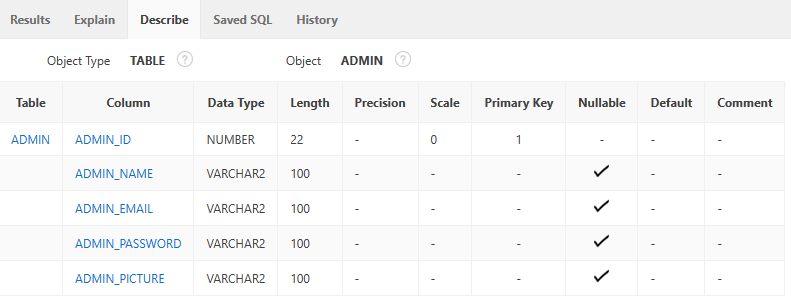
\includegraphics[width=0.8\textwidth]{images/TableDesc/ADMIN.png}
    \caption{Admin table description}
    \label{fig:admin_table}
\end{figure}

% Create Manager table
\begin{lstlisting}[caption={Create Manager table}, label={lst:create_manager}]
    CREATE TABLE Manager (
        Manager_ID INT PRIMARY KEY,
        Manager_Name VARCHAR(100),
        Manager_Email VARCHAR(100),
        Manager_Password VARCHAR(100),
        Manager_Picture VARCHAR(100),
        Manager_Hiredate DATE,
        Admin_ID INT,
        FOREIGN KEY (Admin_id) REFERENCES Manager (Admin_ID)
    );
    \end{lstlisting}

\begin{figure}[h]
    \centering
    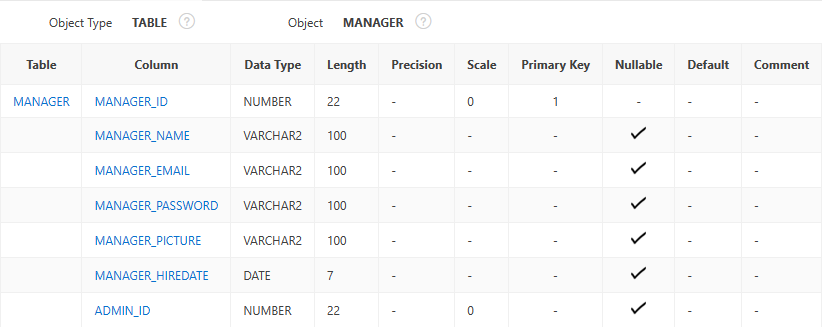
\includegraphics[width=0.8\textwidth]{images/TableDesc/MANAGER.png}
    \caption{Manager table description}
    \label{fig:manger_table}
\end{figure}

% Create Manager Phone table
\begin{lstlisting}[caption={Create Manager Phone table}, label={lst:create_manager_phone}]
    CREATE TABLE Manager_Phone (
        Mp_ID INT PRIMARY KEY,
        Manager_ID INT,
        Manager_Phone VARCHAR(20),
        FOREIGN KEY (Manager_ID) REFERENCES Manager (Manager_ID)
    );
    \end{lstlisting}

\begin{figure}[h]
    \centering
    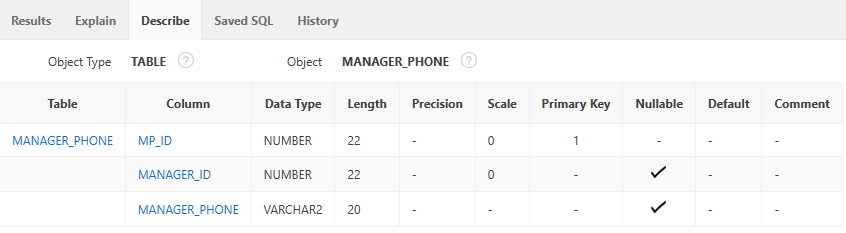
\includegraphics[width=0.8\textwidth]{images/TableDesc/MANAGER_PHONE.png}
    \caption{Manager Phone table description}
    \label{fig:manger_phone_table}
\end{figure}

% Create Finance table
\begin{lstlisting}[caption={Create Finance table}, label={lst:create_finance}]
    CREATE TABLE Finance (
        Finance_ID INT PRIMARY KEY,
        Finance_Account_Number VARCHAR(100),
        Finance_Balance DECIMAL(10, 2),
        Manager_ID INT,
        FOREIGN KEY (Manager_ID) REFERENCES Manager (Manager_ID)
    );
    \end{lstlisting}

\begin{figure}[h]
    \centering
    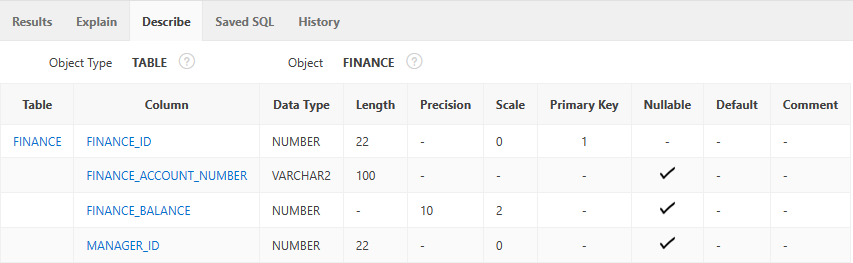
\includegraphics[width=0.8\textwidth]{images/TableDesc/FINANCE.png}
    \caption{Finance table description}
    \label{fig:finance_table}
\end{figure}

% Create Team table
\begin{lstlisting}[caption={Create Team table}, label={lst:create_team}]
    CREATE TABLE Team (
        Team_ID INT PRIMARY KEY,
        Team_Name VARCHAR(100),
        Team_Icon VARCHAR(100),
        Team_Established_Date DATE,
        Team_Country VARCHAR(100),
        Total_Price_Money DECIMAL(10, 2),
        Manager_ID INT,
        FOREIGN KEY (Manager_ID) REFERENCES Manager (Manager_ID)
    );
    \end{lstlisting}
\begin{figure}[H]
    \centering
    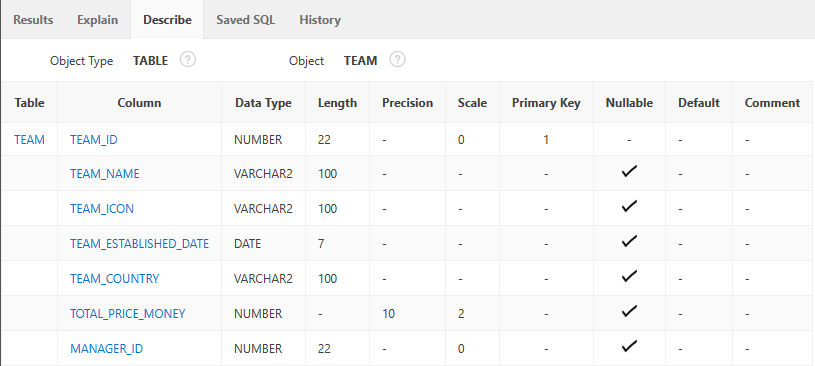
\includegraphics[width=0.8\textwidth]{images/TableDesc/TEAM.png}
    \caption{Team table description}
    \label{fig:team_table}
\end{figure}

% Create Team Winning table
\begin{lstlisting}[caption={Create Team Winning table}, label={lst:create_team_winning}]
    CREATE TABLE Team_Winning (
        Tw_ID INT PRIMARY KEY,
        Team_ID INT,
        Team_Winning VARCHAR(100),
        FOREIGN KEY (Team_ID) REFERENCES Team (Team_ID)
    );
    \end{lstlisting}

\begin{figure}[h]
    \centering
    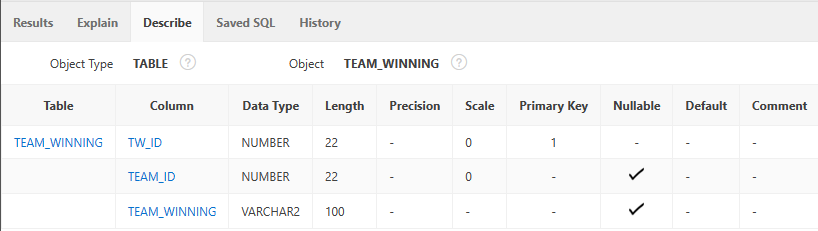
\includegraphics[width=0.8\textwidth]{images/TableDesc/TEAM_WINNING.png}
    \caption{Team Winning table description}
    \label{fig:team_winning_table}
\end{figure}

% Create SocialMedia table
\begin{lstlisting}[caption={Create SocialMedia table}, label={lst:create_socialmedia}]
    CREATE TABLE SocialMedia (
        SocialMedia_ID INT PRIMARY KEY,
        SocialMedia_Name VARCHAR(100),
        SocialMedia_Email VARCHAR(100),
        SocialMedia_Password VARCHAR(100),
        SocialMedia_Picture VARCHAR(100),
        SocialMedia_Hiredate DATE,
        SocialMedia_Salary DECIMAL(10, 2),
        Manager_ID INT,
        FOREIGN KEY (Manager_ID) REFERENCES Manager (Manager_ID)
    );
    \end{lstlisting}
\begin{figure}[H]
    \centering
    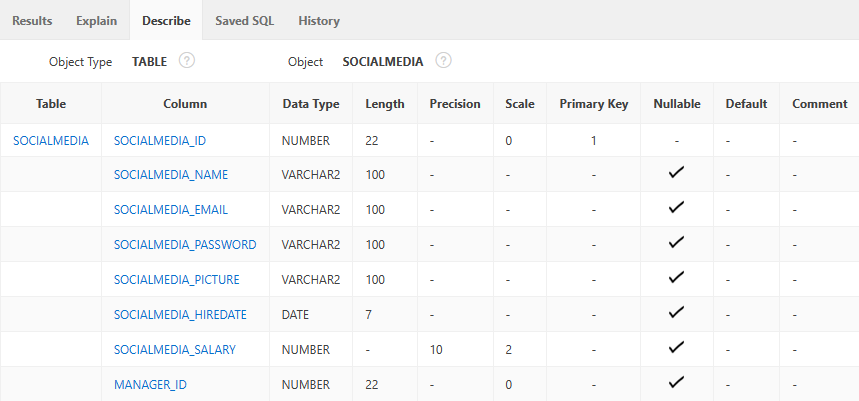
\includegraphics[width=0.8\textwidth]{images/TableDesc/SOCIALMEDIA.png}
    \caption{SocialMedia table description}
    \label{fig:socialmedia_table}
\end{figure}

% Create ContentCreator table
\begin{lstlisting}[caption={Create ContentCreator table}, label={lst:create_contentcreator}]
    CREATE TABLE ContentCreator (
        ContentCreator_ID INT PRIMARY KEY,
        ContentCreator_Name VARCHAR(100),
        ContentCreator_Email VARCHAR(100),
        ContentCreator_Password VARCHAR(100),
        ContentCreator_Picture VARCHAR(100),
        ContentCreator_Hiredate DATE,
        ContentCreator_Salary DECIMAL(10, 2),
        SocialMedia_ID INT,
        FOREIGN KEY (SocialMedia_ID) REFERENCES SocialMedia (SocialMedia_ID)
    );
    \end{lstlisting}

\begin{figure}[H]
    \centering
    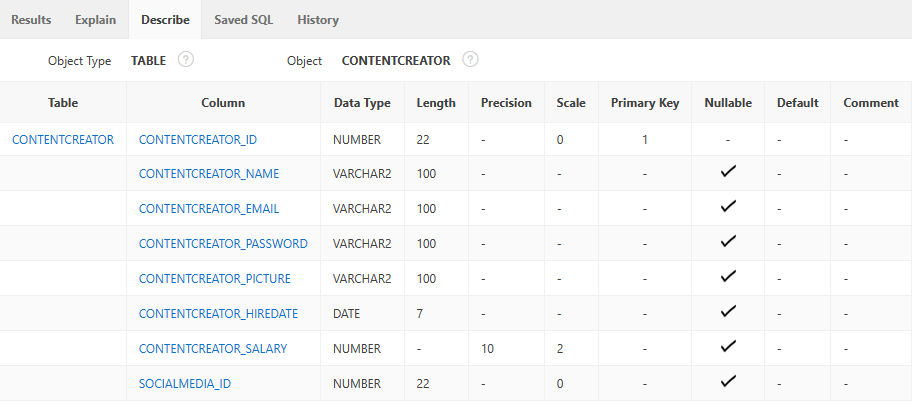
\includegraphics[width=0.8\textwidth]{images/TableDesc/CONTENTCREATOR.png}
    \caption{ContentCreator table description}
    \label{fig:contentcreator_table}
\end{figure}

% Create ContentCreator SocialMedia table
\begin{lstlisting}[caption={Create ContentCreator SocialMedia table}, label={lst:create_contentcreator_socialmedia}]
    CREATE TABLE ContentCreator_SocialMedia (
        Ccs_ID INT PRIMARY KEY,
        ContentCreator_ID INT,
        ContentCreator_Facebook_Link VARCHAR(100),
        ContentCreator_Twitter_Link VARCHAR(100),
        ContentCreator_Instagram_Link VARCHAR(100),
        ContentCreator_Youtube_Link VARCHAR(100),
        FOREIGN KEY (ContentCreator_ID) REFERENCES ContentCreator (ContentCreator_ID)
    );
    \end{lstlisting}
\begin{figure}[H]
    \centering
    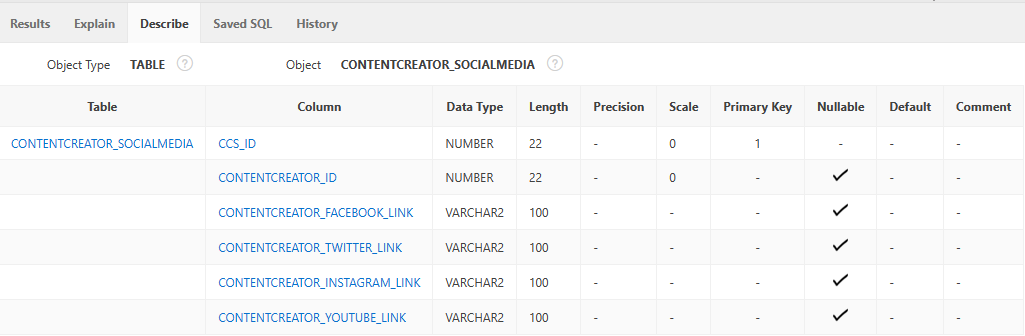
\includegraphics[width=0.8\textwidth]{images/TableDesc/CONTENTCREATOR_SOCIALMEDIA.png}
    \caption{ContentCreator SocialMedia table description}
    \label{fig:contentcreator_socialmedia_table}
\end{figure}
% Create ContentCreator Address table
\begin{lstlisting}[caption={Create ContentCreator Address table}, label={lst:create_contentcreator_address}]
    CREATE TABLE ContentCreator_Address (
        Cca_ID INT PRIMARY KEY,
        ContentCreator_ID INT,
        ContentCreator_Country VARCHAR(100),
        ContentCreator_City VARCHAR(100),
        ContentCreator_Street VARCHAR(100),
        ContentCreator_Zip_Code VARCHAR(20),
        FOREIGN KEY (ContentCreator_ID) REFERENCES ContentCreator (ContentCreator_ID)
    );
    \end{lstlisting}
\begin{figure}[H]
    \centering
    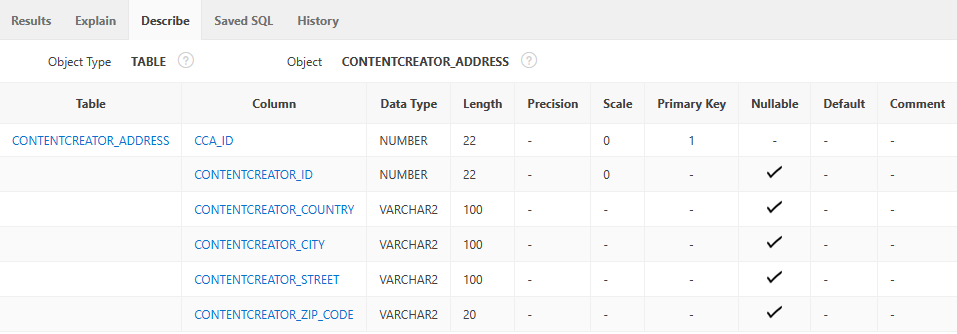
\includegraphics[width=0.8\textwidth]{images/TableDesc/CONTENTCREATOR_ADDRESS.png}
    \caption{ContentCreator Address table description}
    \label{fig:contentcreator_address_table}
\end{figure}
% Create ContentCreator Phone table
\begin{lstlisting}[caption={Create ContentCreator Phone table}, label={lst:create_contentcreator_phone}]
    CREATE TABLE ContentCreator_Phone (
        Ccp_ID INT PRIMARY KEY,
        ContentCreator_ID INT,
        ContentCreator_Phone VARCHAR(20),
        FOREIGN KEY (ContentCreator_ID) REFERENCES ContentCreator (ContentCreator_ID)
    );
    \end{lstlisting}
\clearpage
% Create SocialMedia Phone table
\begin{lstlisting}[caption={Create SocialMedia Phone table}, label={lst:create_socialmedia_phone}]
    CREATE TABLE SocialMedia_Phone (
        Smp_ID INT PRIMARY KEY,
        SocialMedia_ID INT,
        SocialMedia_Phone VARCHAR(20),
        FOREIGN KEY (SocialMedia_ID) REFERENCES SocialMedia (SocialMedia_ID)
    );
    \end{lstlisting}
\begin{figure}[H]
    \centering
    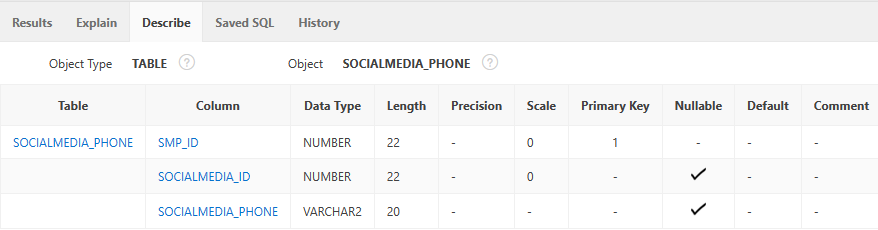
\includegraphics[width=0.8\textwidth]{images/TableDesc/SOCIALMEDIA_PHONE.png}
    \caption{SocialMedia Phone table description}
    \label{fig:socialmedia_phone_table}
\end{figure}
% Create Organization table
\begin{lstlisting}[caption={Create Organization table}, label={lst:create_organization}]
    CREATE TABLE Organization (
        Organization_ID INT PRIMARY KEY,
        Organization_Name VARCHAR(100),
        Organization_Email VARCHAR(100),
        Organization_Password VARCHAR(100),
        Organization_Picture VARCHAR(100),
        Organization_Phone VARCHAR(20),
        Finance_ID INT,
        FOREIGN KEY (Finance_ID) REFERENCES Finance (Finance_ID)
    );
    \end{lstlisting}
\begin{figure}[H]
    \centering
    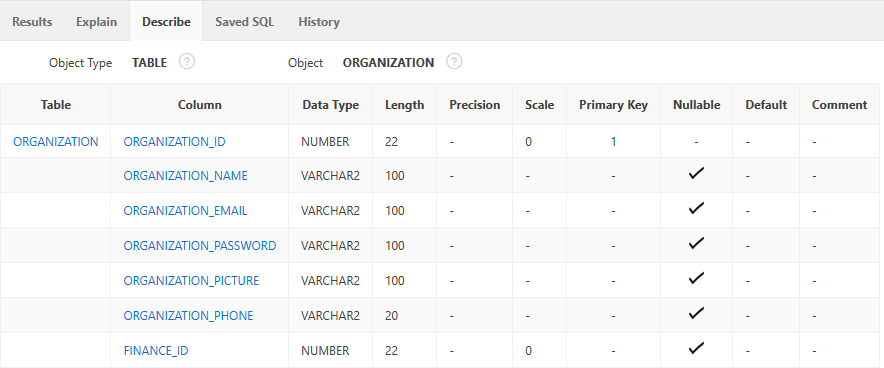
\includegraphics[width=0.8\textwidth]{images/TableDesc/ORGANIZATION.png}
    \caption{Organization table description}
    \label{fig:organization_table}
\end{figure}
% Create Organization Phone table
\begin{lstlisting}[caption={Create Organization Phone table}, label={lst:create_organization_phone}]
    CREATE TABLE Organization_Phone (
        Op_ID INT PRIMARY KEY,
        Organization_ID INT,
        Organization_Phone VARCHAR(20),
        FOREIGN KEY (Organization_ID) REFERENCES Organization (Organization_ID)
    );
    \end{lstlisting}
\begin{figure}[H]
    \centering
    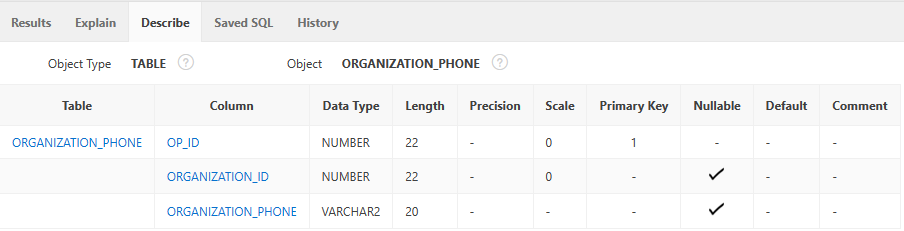
\includegraphics[width=0.8\textwidth]{images/TableDesc/ORGANIZATION_PHONE.png}
    \caption{Organization Phone table description}
    \label{fig:organization_phone_table}
\end{figure}
% Create Player table
\begin{lstlisting}[caption={Create Player table}, label={lst:create_player}]
    CREATE TABLE Player (
        Player_ID INT PRIMARY KEY,
        Player_Name VARCHAR(100),
        Player_Email VARCHAR(100),
        Player_Password VARCHAR(100),
        Player_Picture VARCHAR(100),
        Player_JoinDate DATE,
        Player_Salary DECIMAL(10, 2),
        Player_Play_Hours INT,
        Player_DOB DATE
    );
    \end{lstlisting}
\begin{figure}[H]
    \centering
    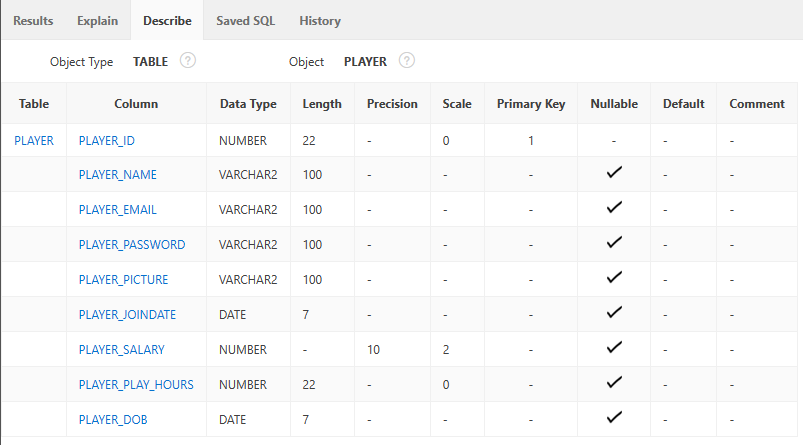
\includegraphics[width=0.8\textwidth]{images/TableDesc/PLAYER.png}
    \caption{Player table description}
    \label{fig:player_table}
\end{figure}
% Create Player Address table
\begin{lstlisting}[caption={Create Player Address table}, label={lst:create_player_address}]
    CREATE TABLE Player_Address (
        Pa_ID INT PRIMARY KEY,
        Player_ID INT,
        Player_Country VARCHAR(100),
        Player_City VARCHAR(100),
        Player_Street VARCHAR(100),
        Player_Zip_Code VARCHAR(20),
        FOREIGN KEY (Player_ID) REFERENCES Player (Player_ID)
    );
    \end{lstlisting}
\begin{figure}[H]
    \centering
    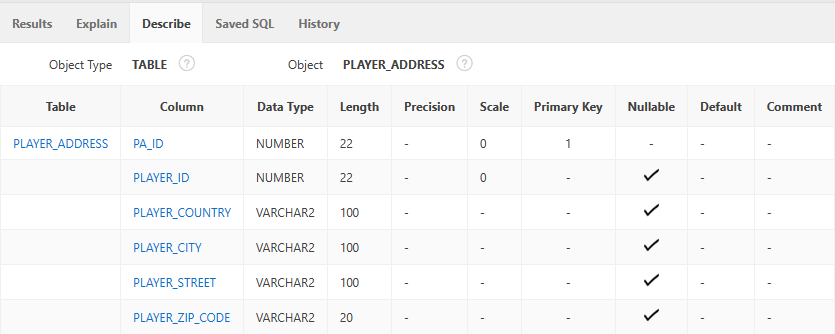
\includegraphics[width=0.8\textwidth]{images/TableDesc/PLAYER_ADDRESS.png}
    \caption{Player Address table description}
    \label{fig:player_address_table}
\end{figure}
% Create Player Social Link table
\begin{lstlisting}[caption={Create Player Social Link table}, label={lst:create_player_social_link}]
    CREATE TABLE Player_Social_Link (
        Psl_ID INT PRIMARY KEY,
        Player_ID INT,
        Player_Facebook_Link VARCHAR(100),
        Player_Instagram_Link VARCHAR(100),
        Player_Twitter_Link VARCHAR(100),
        Player_Youtube_Link VARCHAR(100),
        FOREIGN KEY (Player_ID) REFERENCES Player (Player_ID)
    );
    \end{lstlisting}
\begin{figure}[H]
    \centering
    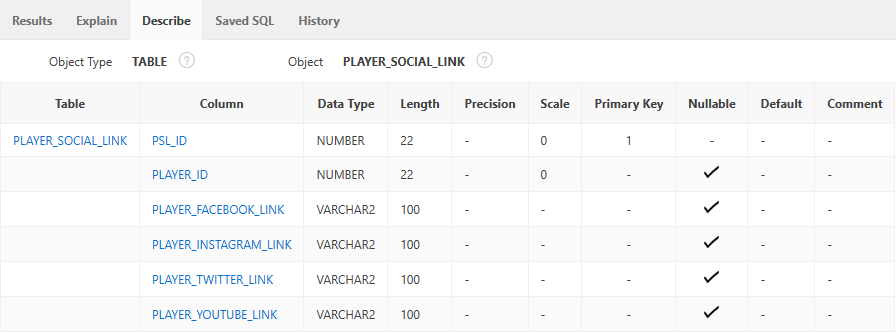
\includegraphics[width=0.8\textwidth]{images/TableDesc/PLAYER_SOCIAL_LINK.png}
    \caption{Player Social Link table description}
    \label{fig:player_social_link_table}
\end{figure}
\clearpage
% Create Player Phone table
\begin{lstlisting}[caption={Create Player Phone table}, label={lst:create_player_phone}]
    CREATE TABLE Player_Phone (
        Pp_ID INT PRIMARY KEY,
        Player_ID INT,
        Player_Phone VARCHAR(20),
        FOREIGN KEY (Player_ID) REFERENCES Player (Player_ID)
    );
    \end{lstlisting}
\begin{figure}[H]
    \centering
    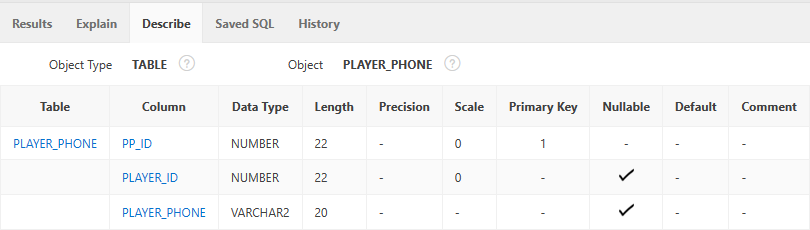
\includegraphics[width=0.8\textwidth]{images/TableDesc/PLAYER_PHONE.png}
    \caption{Player Phone table description}
    \label{fig:player_phone_table}
\end{figure}
% Create Player Winning table
\begin{lstlisting}[caption={Create Player Winning table}, label={lst:create_player_winning}]
    CREATE TABLE Player_Winning (
        Pw_ID INT PRIMARY KEY,
        Player_ID INT,
        Player_Winning VARCHAR(100),
        FOREIGN KEY (Player_ID) REFERENCES Player (Player_ID)
    );
    \end{lstlisting}
\begin{figure}[H]
    \centering
    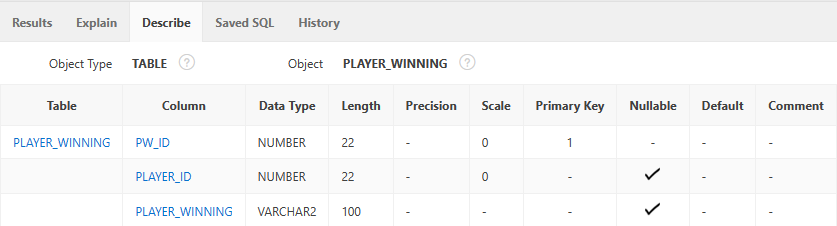
\includegraphics[width=0.8\textwidth]{images/TableDesc/PLAYER_WINNING.png}
    \caption{Player Winning table description}
    \label{fig:player_winning_table}
\end{figure}
% Create Player Team table
\begin{lstlisting}[caption={Create Player Team table}, label={lst:create_player_team}]
    CREATE TABLE Player_Team (
        Pt_ID INT PRIMARY KEY,
        Player_ID INT,
        Team_ID INT,
        FOREIGN KEY (Player_ID) REFERENCES Player (Player_ID),
        FOREIGN KEY (Team_ID) REFERENCES Team (Team_ID)
    );
    \end{lstlisting}
\begin{figure}[H]
    \centering
    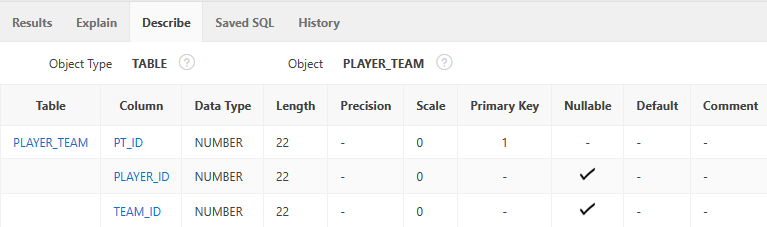
\includegraphics[width=0.8\textwidth]{images/TableDesc/PLAYER_TEAM.png}
    \caption{Player Team table description}
    \label{fig:player_team_table}
\end{figure}
% Create Tournament table
\begin{lstlisting}[caption={Create Tournament table}, label={lst:create_tournament}]
    CREATE TABLE Tournament (
        Tournament_ID INT PRIMARY KEY,
        Tournament_Name VARCHAR(100),
        Tournament_StartingDate DATE,
        Tournament_EndingDate DATE,
        Tournament_Location VARCHAR(100),
        Tournament_Prize_Pool DECIMAL(10, 2),
        Organization_ID INT,
        FOREIGN KEY (Organization_ID) REFERENCES Organization (Organization_ID)
    );
    \end{lstlisting}
\begin{figure}[H]
    \centering
    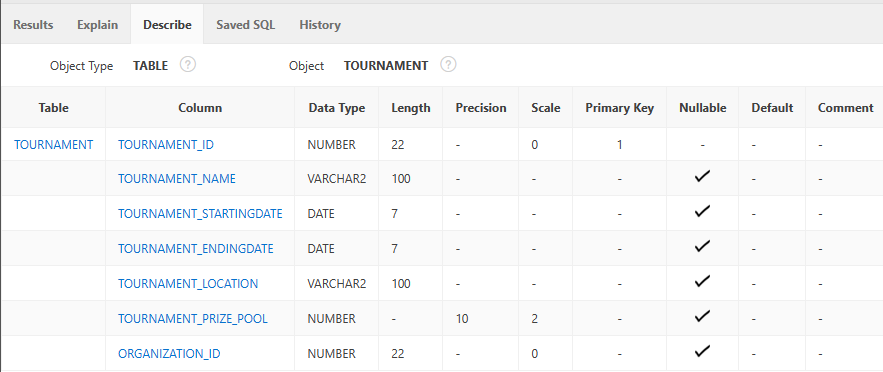
\includegraphics[width=0.8\textwidth]{images/TableDesc/TOURNAMENT.png}
    \caption{Tournament table description}
    \label{fig:tournament_table}
\end{figure}
% Create Record table
\begin{lstlisting}[caption={Create Record table}, label={lst:create_record}]
    CREATE TABLE Record (
        Record_ID INT PRIMARY KEY,
        Record_Date DATE,
        Record_Price_Pool DECIMAL(10, 2),
        Tournament_ID INT,
        FOREIGN KEY (Tournament_ID) REFERENCES Tournament (Tournament_ID)
    );
    \end{lstlisting}
\begin{figure}[H]
    \centering
    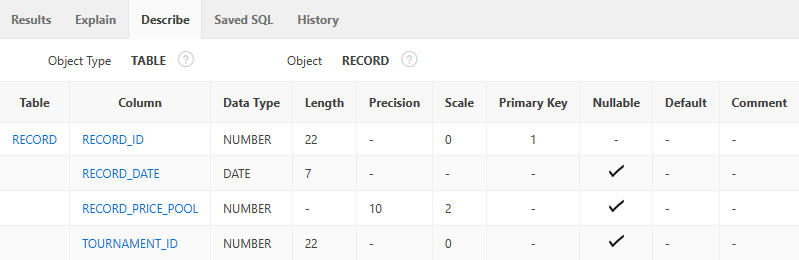
\includegraphics[width=0.8\textwidth]{images/TableDesc/RECORD.png}
    \caption{Record table description}
    \label{fig:record_table}
\end{figure}

% Create Game table
\begin{lstlisting}[caption={Create Game table}, label={lst:create_game}]
    CREATE TABLE Game (
        Game_ID INT PRIMARY KEY,
        Game_Name VARCHAR(100),
        Game_Icon VARCHAR(100),
        Game_ReleaseDate DATE,
        Game_Platform VARCHAR(100),
        Game_Price_Pool DECIMAL(10, 2),
        Game_Genre VARCHAR(100),
        Game_Publisher VARCHAR(100)
    );
    \end{lstlisting}
\begin{figure}[H]
    \centering
    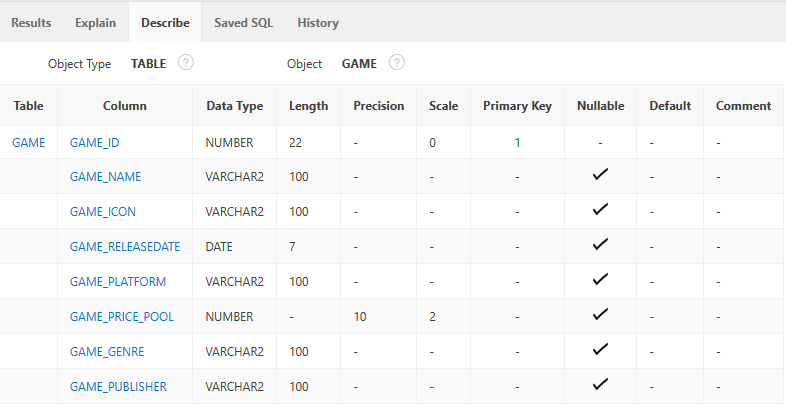
\includegraphics[width=0.8\textwidth]{images/TableDesc/GAME.png}
    \caption{Game table description}
    \label{fig:game_table}
\end{figure}

% Create Tournament Game table
\begin{lstlisting}[caption={Create Tournament Game table}, label={lst:create_tournament_game}]
    CREATE TABLE Tournament_Game (
        Tournament_ID INT,
        Game_ID INT,
        PRIMARY KEY (Tournament_ID, Game_ID),
        FOREIGN KEY (Tournament_ID) REFERENCES Tournament (Tournament_ID),
        FOREIGN KEY (Game_ID) REFERENCES Game (Game_ID)
    );
    \end{lstlisting}
\begin{figure}[H]
    \centering
    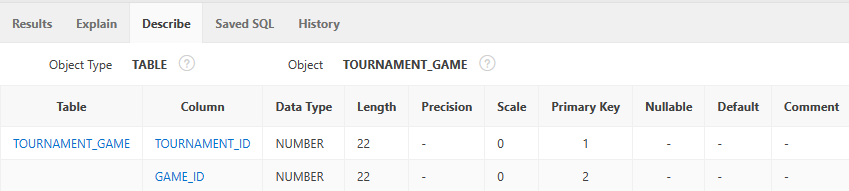
\includegraphics[width=0.8\textwidth]{images/TableDesc/TOURNAMENT_GAME.png}
    \caption{Tournament Game table description}
    \label{fig:tournament_game_table}
\end{figure}
% Create Organization Tournament table
\begin{lstlisting}[caption={Create Organization Tournament table}, label={lst:create_organization_tournament}]
    CREATE TABLE Organization_Tournament (
        Organization_ID INT,
        Tournament_ID INT,
        PRIMARY KEY (Organization_ID, Tournament_ID),
        FOREIGN KEY (Organization_ID) REFERENCES Organization (Organization_ID),
        FOREIGN KEY (Tournament_ID) REFERENCES Tournament (Tournament_ID)
    );
    \end{lstlisting}
\begin{figure}[H]
    \centering
    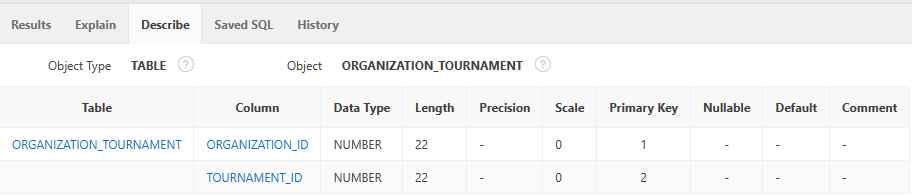
\includegraphics[width=0.8\textwidth]{images/TableDesc/ORGANIZATION_TOURNAMENT.png}
    \caption{Organization Tournament table description}
    \label{fig:organization_tournament_table}
\end{figure}
\clearpage
% Create Team Game table
\begin{lstlisting}[caption={Create Team Game table}, label={lst:create_team_game}]
    CREATE TABLE Team_Game (
        Team_ID INT,
        Game_ID INT,
        PRIMARY KEY (Team_ID, Game_ID),
        FOREIGN KEY (Team_ID) REFERENCES Team (Team_ID),
        FOREIGN KEY (Game_ID) REFERENCES Game (Game_ID)
    );
    \end{lstlisting}
\begin{figure}[H]
    \centering
    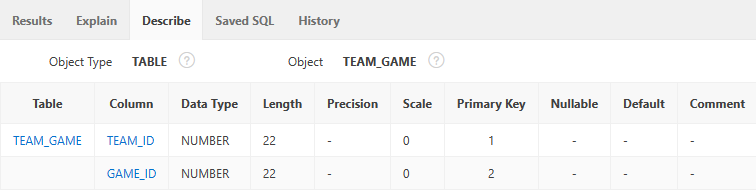
\includegraphics[width=0.8\textwidth]{images/TableDesc/TEAM_GAME.png}
    \caption{Team Game table description}
    \label{fig:team_game_table}
\end{figure}
% Create Company table
\begin{lstlisting}[caption={Create Company table}, label={lst:create_company}]
    CREATE TABLE Company (
        Company_ID INT PRIMARY KEY,
        Company_Name VARCHAR(100),
        Company_Email VARCHAR(100),
        Company_Picture VARCHAR(100),
        Company_Phone VARCHAR(20),
        Company_Location VARCHAR(100)
    );
    \end{lstlisting}
\begin{figure}[H]
    \centering
    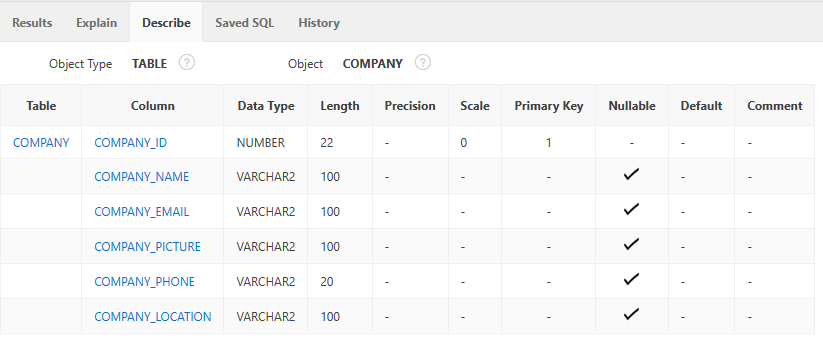
\includegraphics[width=0.8\textwidth]{images/TableDesc/COMPANY.png}
    \caption{Company table description}
    \label{fig:company_table}
\end{figure}
% Create Company Phone table
\begin{lstlisting}[caption={Create Company Phone table}, label={lst:create_company_phone}]
    CREATE TABLE Company_Phone (
        Company_ID INT,
        Company_Phone VARCHAR(20),
        PRIMARY KEY (Company_ID, Company_Phone),
        FOREIGN KEY (Company_ID) REFERENCES Company (Company_ID)
    );
    \end{lstlisting}
\begin{figure}[H]
    \centering
    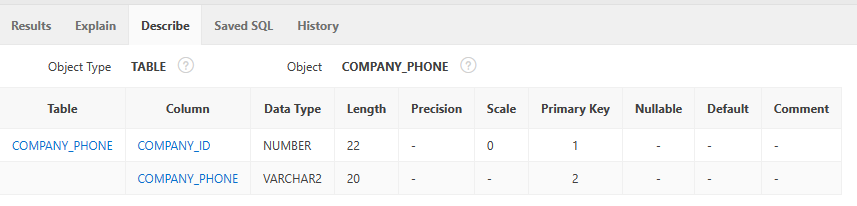
\includegraphics[width=0.8\textwidth]{images/TableDesc/CompanyPhone.png}
    \caption{Company Phone table description}
    \label{fig:company_phone_table}
\end{figure}
% Create Organization Company table
\begin{lstlisting}[caption={Create Organization Company table}, label={lst:create_organization_company}]
    CREATE TABLE Organization_Company (
        Organization_ID INT,
        Company_ID INT,
        PRIMARY KEY (Organization_ID, Company_ID),
        FOREIGN KEY (Organization_ID) REFERENCES Organization (Organization_ID),
        FOREIGN KEY (Company_ID) REFERENCES Company (Company_ID)
    );
    \end{lstlisting}
\begin{figure}[H]
    \centering
    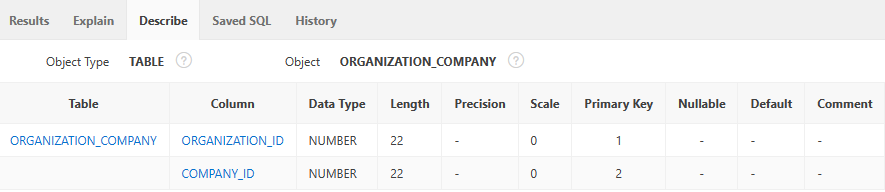
\includegraphics[width=0.8\textwidth]{images/TableDesc/ORGANIZATION_COMPANY.png}
    \caption{Organization Company table description}
    \label{fig:organization_company_table}
\end{figure}
% Create Team Company table
\begin{lstlisting}[caption={Create Team Company table}, label={lst:create_team_company}]
    CREATE TABLE Team_Company (
        Team_ID INT,
        Company_ID INT,
        PRIMARY KEY (Team_ID, Company_ID),
        FOREIGN KEY (Team_ID) REFERENCES Team (Team_ID),
        FOREIGN KEY (Company_ID) REFERENCES Company (Company_ID)
    );
    \end{lstlisting}
\begin{figure}[H]
    \centering
    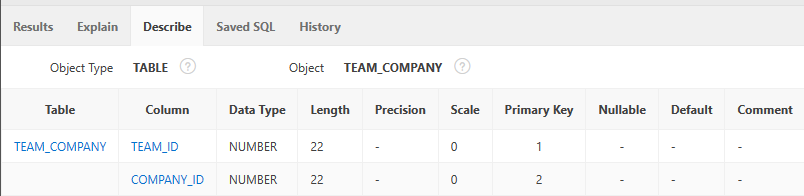
\includegraphics[width=1\textwidth]{images/TableDesc/TEAM_COMPANY.png}
    \caption{Team Company table description}
    \label{fig:team_company_table}
\end{figure}
\clearpage
